\subsection{Fran's results}
\begin{algorithm}
\caption{Tree to formula -- $Tree2STL(\cdot)$}
\label{alg:tree2formula}
\DontPrintSemicolon
\KwIn{$node$ -- Starting node of a tree}
\KwOut{Formula}
\BlankLine

\uIf{$node$ is $leaf$}{
    \Return{$\True$}
}

$\phi \asgn$ formula associated with $node$

\uIf{$node.right$ is $leaf$}{
    \Return{$\phi \andltl Tree2STL(node.left)$}
}\Else{
    \Return{$(\phi \andltl Tree2STL(node.left)) \orltl (\notltl \phi \andltl Tree2STL(node.right))$}
}
\end{algorithm}

We implemented and tested two different instances of Alg.\ref{alg:inf}, $I_1$ and $I_2$, defined by the choice of parameters given in Table \ref{tab:inst}. In the case of $I_1$, the implementation was done in Matlab using standard libraries, using the simulated annealing optimization method and run on a 3.5 GHz processor with 16 GB RAM. As for $I_2$, we used the SciPy library for Python, solving the optimization problem with its implementation of the differential evolution algorithm, and we tested it on similar hardware.


\begin{table}
    \begin{tabular}{|c|c|c|p{3cm}|}
    \hline
    Instance & Primitives & Impurity & Stopping \\ \hline
    $I_1$ & $\CA{P}_1$ & $MG_r$ & Majority class rate >0.99, Depth >4 \\ \hline
    $I_2$ & $\CA{P}_2$ & $IG_r$ & Depth >3 \\ \hline
\end{tabular}
\caption{Algorithm parameters}
\label{tab:inst}
\end{table}

Maritime surveillance

We tested the $I_2$ instance using a non stratified 10-fold cross-validation with a random permutation of the data set, obtaining a mean misclassification rate of 0.007 with a standard deviation of 0.008 and a run time of about 4 hours per split. A (simplified) sample formula learned from one of the runs is:

\begin{equation}
    \label{eq:nav2}
\begin{aligned}
    \phi & = ( \phi_1 \andltl (\notltl \phi_2 \orltl (\phi_2 \andltl \notltl \phi_3))) \orltl (\notltl \phi_1 \andltl (\phi_4 \andltl \phi_5)) \\
    \phi_1 & = \Always_{[199.70, 297.27)} \Event_{[0.00, 0.05)} (x \le 23.60) \\
    \phi_2 & = \Always_{[4.47, 16.64)} \Event_{[0.00, 198.73)} (y \le 24.20) \\
    \phi_3 & = \Always_{[34.40, 52.89)} \Event_{[0.00, 61.74)} (y \le 19.62) \\
    \phi_4 & = \Always_{[30.96, 37.88)} \Event_{[0.00, 250.37)} (x \le 36.60) \\
    \phi_5 & = \Always_{[62.76, 253.23)} \Event_{[0.00, 41.07)} (y \le 29.90)
\end{aligned}
\end{equation}

We can see in Figure~\ref{fig:navalresults} how the thresholds for $\phi_1$ and $\phi_2$ capture the key features of the data set. Notice also the insight we can gain from their plain English translation: "Normal vessels' $x$ coordinate is below 23.6 during the last 100 seconds, i.e., they approach and remain at the port" and "normal vessels' $y$ coordinate never go below 24.2, i.e., they don't approach the island". It is worth mentioning the second term of the outer disjunction in $\phi$, as it highlights a feature of the data set difficult to spot on the figures: some normal vessels don't reach the port (inspecting the data set, some normal traces stop right after crossing the passage). As usual when employing decision trees, deeper formulae focus on finer details of the data set.

\begin{figure}
    \centering
    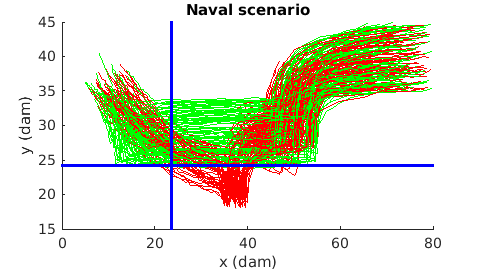
\includegraphics[width=1.0\columnwidth]{naval_res}
    \caption{A sample of the naval surveillance data set with normal trajectories shown in green and anomalous trajectories in red. We show in blue the boundaries of $\phi_1$ and $\phi_2$ in \ref{eq:nav2}.}
    \label{fig:navalresults}
\end{figure}

In the case of $I_1$, we tested it with a single random split of {\color{red}X} training traces and {\color{red}X} validation traces. We obtained for this experiment a misclassification rate of {\color{red}X}, with a run time of about {\color{red}X} minutes and the following formula:

\begin{equation}
    \label{eq:nav1}
\begin{aligned}
    \phi & = (\phi_1 \andltl (\phi_2 \andltl \phi_3 )  \orltl ( \notltl \phi_1 \andltl (\phi_4 \andltl \phi_5 )) \\
    \phi_1 & = \Always_{[94.6,300)} (y\le35.3) \\
    \phi_2 & = \Always_{[0,300)} (y>23) \\
    \phi_3 & = \Always_{[298,300)} (x\le25.9) \\
    \phi_4 & = \Always_{[182,300)} (x\le19.6) \\
    \phi_5 & = \Always_{[0,51.6)} (x>42.6)
\end{aligned}
\end{equation}

Note the similarity between the subformulas $\phi_2$ or between $\phi_1$ and $\phi_3$ in \ref{eq:nav2} and \ref{eq:nav1} respectively.

Fuel control

In this scenario, we tested both instances using only the {\color{red} X and Y} variables of the data set. We performed a similar cross-validation for $I_2$\footnote{Due to time constraints, we only report here the results for the first three splits}, resulting in a mean misclassification rate of 0.031 with a standard deviation of 0.008 and a run time of about 15 hours per split. A sample formula is:

\begin{equation}
    \label{eq:fuel2}
\begin{aligned}
    \phi & =  \notltl \phi_1 \andltl \phi_2 \andltl \phi_3 \\
    \phi_1 & = \Event_{[1.85, 58.70)} \Always_{[0.00, 0.57)} (x_0 \le 0.13) \\
    \phi_2 & = \Always_{[11.35, 59.55)} \Event_{[0.00, 0.03)} (x_0 \le 0.99) \\
    \phi_3 & = \Always_{[1.65, 58.89)} \Event_{[0.00, 0.44)} (x_1 \le 0.90) \\
\end{aligned}
\end{equation}

Notice in this case how the resulting subformulas are equivalent to level 1 primitives, suggesting that $\CA{P}_2$ is an overly complicated set of primitives.

Regarding $I_1$, we obtained a misclassification rate of {\color{red} X} for a run time of {\color{red} X} minutes. The resulting formula is the following:


\begin{equation}
    \label{eq:fuel1}
\begin{aligned}
    \phi & = \phi_1 \andltl (\phi_2 \andltl (\phi_3 \andltl \phi_4)) \\
    \phi_1 & = \Always_{[0,59.7)} (x_{2}>-0.563) \\
    \phi_2 & = \Always_{[0,59.7)} (x_{2}\le1.91) \\
    \phi_3 & = \Always_{[0,59.7)} (x_{1}>-0.819) \\
    \phi_4 & = \Always_{[23.7,59.7)} (x_{1}\le1.78)
\end{aligned}
\end{equation}

{\color{blue} Fix variable names in fuel control formulas. I'm calling $\phi$ to all the formulas, we may want to change that}
